% !TeX root = 00P2_cep_semantics.tex

\section{Envelopes and Attestations as Natural Transformations}
\label{sec:envelopes}

CEP record envelopes, including schema references, revision metadata,
timestamps, and cryptographic attestations, are not merely auxiliary
fields.
They impose a structural layer that is functorial: every payload
can be given an envelope, and every valid update to a payload induces a
corresponding update to its envelope.
This section formalizes that layer
using functors and natural transformations.

% ------------------------------------------------------------
\subsection{Envelopes as Functors}
% ------------------------------------------------------------

Let $\mathbf{P}$ denote the category of \emph{raw payloads}, whose
objects are unenveloped CEP payloads (entities, relationships, and
exchanges), and whose morphisms are valid payload-level transformations
(e.g., updates, amendments, or partial recomputations) that do not yet
touch attestation or revision metadata.

Let $\mathbf{E}$ denote the category of \emph{enveloped records}, in
which each object consists of a payload together with its envelope, and
morphisms are the provenance-preserving transformations defined in
Section~\ref{sec:cep}.

We define the \emph{enveloping functor}
\begin{equation}
  \mathcal{E} : \mathbf{P} \to \mathbf{E}
\end{equation}
that assigns to each payload $P$ an enveloped record $\mathcal{E}(P)$.
The functor:
\begin{itemize}
  \item injects the schema reference,
  \item initializes revision and lifecycle fields,
  \item creates timestamps for observation and validity,
  \item embeds the canonical (identity-bearing) fields.
\end{itemize}

On morphisms, $\mathcal{E}(f)$ augments a payload-level update
$f : P \to P'$ with corresponding envelope updates that preserve schema
validity, revision monotonicity, and identifier invariance.

Thus, the enveloping process is not an ad hoc transformation but a
strictly functorial lift from payload space to the full CEP record space.

% ------------------------------------------------------------
\subsection{Attestations as Natural Transformations}
% ------------------------------------------------------------

Let $\mathcal{E}'$ be a functor
\[
  \mathcal{E}' : \mathbf{P} \to \mathbf{E}
\]
representing the construction of \emph{attested envelopes}, where each
payload $P$ receives an envelope that incorporates a cryptographic
validation step (digital signature, proof-of-origin, or other attestation
mechanism).
As with $\mathcal{E}$, this functor acts on both objects and morphisms.

An attestation operation is then modeled as a \emph{natural
  transformation}
\[
  \alpha : \mathcal{E} \Longrightarrow \mathcal{E}'.
\]
For each payload $P$, the component
\[
  \alpha_P : \mathcal{E}(P) \to \mathcal{E}'(P)
\]
corresponds to the application of a cryptographic attestation method
(e.g., signing, sealing, notarizing) to the envelope of $P$.

Naturality requires that for every payload morphism $f : P \to P'$ in
$\mathbf{P}$, the following square commutes:
\[
  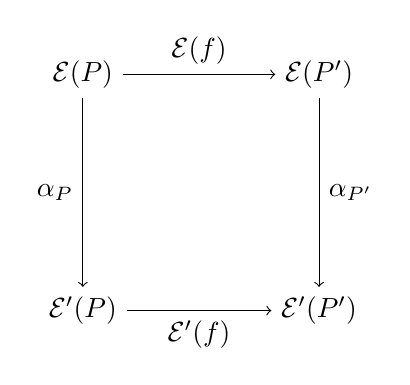
\begin{tikzpicture}[node distance=3cm]
    \node (EP) {$\mathcal{E}(P)$};
    \node (EPP) [right of=EP] {$\mathcal{E}(P')$};
    \node (EPa) [below of=EP] {$\mathcal{E}'(P)$};
    \node (EPPa) [right of=EPa] {$\mathcal{E}'(P')$};

    \draw[->] (EP) -- node[above] {$\mathcal{E}(f)$} (EPP);
    \draw[->] (EP) -- node[left] {$\alpha_P$} (EPa);
    \draw[->] (EPP) -- node[right] {$\alpha_{P'}$} (EPPa);
    \draw[->] (EPa) -- node[below] {$\mathcal{E}'(f)$} (EPPa);
  \end{tikzpicture}
\]

\FigureCallout{Attestations as Natural Transformations (Provenance Commutativity)}{
  The naturality of $\alpha$ ensures that the act of attesting
  ($\alpha_P$) commutes with the act of transforming the payload
  ($\mathcal{E}(f)$).
  This formalizes the requirement that provenance chains remain consistent:
  an attestation applied before or after an update must yield envelopes
  related in a predictable, structure-preserving manner.
}

This formalizes CEP's design principle that attestations do not break
transformations and transformations do not invalidate attestations.

% ------------------------------------------------------------
\subsection{Revision Monotonicity as a Functorial Constraint}
% ------------------------------------------------------------

Let $(\mathbb{N}, \le)$ denote the natural numbers ordered by the usual
non-decreasing relation.
Revision numbers in CEP form a functor:
\[
  \mathrm{Rev} : \mathbf{E} \to (\mathbb{N}, \le),
\]
which assigns to each enveloped record its revision number and to each
morphism $R \to R'$ the corresponding order-preserving mapping
$\mathrm{Rev}(R) \le \mathrm{Rev}(R')$.

Thus, revision monotonicity is not merely a rule but a categorical
invariant: all CEP morphisms must map to monotone arrows in
$(\mathbb{N}, \le)$.
This captures the immutability and forward-only
progression of the revision field as a semantic constraint enforced at
the categorical level.

% ------------------------------------------------------------
\subsection{Envelopes as a Comonad}
% ------------------------------------------------------------

The enveloping process admits an alternative and illuminating
interpretation:
it behaves comonadically when viewed as a context
constructor on payloads~\citep{maclane1971categories,awodey2010category}.

Concretely, consider a category $\mathbf{P}_{\mathsf{env}}$ whose
objects are payloads together with their envelopes, but where we
regard the payload component as primary and the envelope as context.
On this category, an endofunctor
\[
  \mathsf{C} : \mathbf{P}_{\mathsf{env}} \to \mathbf{P}_{\mathsf{env}}
\]
can be defined that ``adds context'' in the sense of enriching a record
with its envelope structure.

A comonad $(\mathsf{C}, \varepsilon, \delta)$ consists of:
\begin{itemize}
  \item a functor $\mathsf{C} : \mathbf{P}_{\mathsf{env}} \to \mathbf{P}_{\mathsf{env}}$,
  \item a counit $\varepsilon : \mathsf{C} \Rightarrow \mathrm{Id}$,
  \item a comultiplication
        $\delta : \mathsf{C} \Rightarrow \mathsf{C}\mathsf{C}$,
\end{itemize}
satisfying standard coassociativity and counitality laws.

In CEP:
\begin{itemize}
  \item $\mathsf{C}(P)$ is the ``contextualized'' version of $P$,
        carrying its envelope,
  \item $\varepsilon$ extracts the underlying payload from its envelope,
  \item $\delta$ enriches a record with its own envelope again,
        representing recursive contextualization (e.g., envelopes of envelopes).
\end{itemize}

This perspective aligns CEP envelopes with the comonadic
interpretation of contextual data in database theory~\citep{spivak2014category}.

% ------------------------------------------------------------
\subsection{Attestations as a Cartesian Natural Transformation}
% ------------------------------------------------------------

Not all natural transformations preserve the limit structure needed for
record-level consistency.
CEP attestations must preserve pullbacks:
they cannot break joins or invalidate prior provenance.

Thus we refine $\alpha : \mathcal{E} \Rightarrow \mathcal{E}'$ to be a
\emph{cartesian natural transformation}, meaning that each naturality
square is a pullback square.

Formally, for every $f : P \to P'$,
\[
  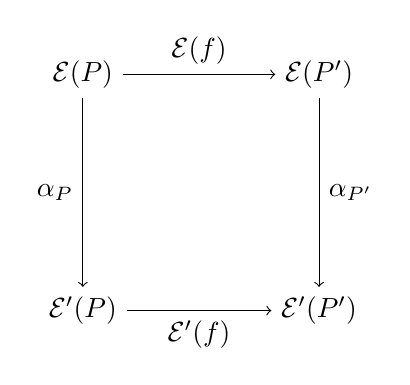
\begin{tikzpicture}[node distance=3cm]
    \node (EP) {$\mathcal{E}(P)$};
    \node (EPP) [right of=EP] {$\mathcal{E}(P')$};
    \node (EPa) [below of=EP] {$\mathcal{E}'(P)$};
    \node (EPPa) [right of=EPa] {$\mathcal{E}'(P')$};

    \draw[->] (EP) -- node[above] {$\mathcal{E}(f)$} (EPP);
    \draw[->] (EP) -- node[left] {$\alpha_P$} (EPa);
    \draw[->] (EPP) -- node[right] {$\alpha_{P'}$} (EPPa);
    \draw[->] (EPa) -- node[below] {$\mathcal{E}'(f)$} (EPPa);
  \end{tikzpicture}
\]
is required to be a pullback.

Cartesianness ensures:
\begin{itemize}
  \item attestations preserve joins,
  \item no new contradictions arise under $\alpha$,
  \item provenance behaves consistently across merges.
\end{itemize}

This matches CEP's requirement that attestations cannot ``detach'' from
the record state they certify.

% ------------------------------------------------------------
\subsection{CEP as a Fibred Category}
% ------------------------------------------------------------

Let $\mathbf{Sch}$ denote the category of CEP schemas and controlled
vocabulary URIs.
Each CEP record is typed by a schema element, giving rise to a functor:
\[
  \pi : \mathbf{CEP} \to \mathbf{Sch}.
\]

We interpret $\pi$ as a \emph{fibration}: for any morphism
$s : S \to S'$ in $\mathbf{Sch}$ and any record $R'$ over $S'$, there
exists a \emph{cartesian lifting} describing the induced transformation
on record instances.

This validates two core CEP invariants:
\begin{itemize}
  \item type-consistent updates always exist,
  \item vocabulary and schema evolution propagate along cartesian liftings.
\end{itemize}

The fibred structure provides the mathematical foundation for version
migration and schema evolution.

% ------------------------------------------------------------
\subsection{Relation to W3C PROV}
% ------------------------------------------------------------


CEP attestation components align directly with PROV-DM constructs:
\begin{center}
  \begin{tabular}{ll}
    \toprule
    CEP Component                 & PROV Construct                                      \\
    \midrule
    \texttt{attestorId}           & \texttt{prov:Agent}                                 \\
    \texttt{attestationTimestamp} & \texttt{prov:Generation} / \texttt{prov:Start}      \\
    \texttt{proofType}            & \texttt{prov:Activity} type                         \\
    \texttt{proofPurpose}         & \texttt{prov:Plan} or \texttt{prov:Role}            \\
    \texttt{proofValue}           & \texttt{prov:Entity} / \texttt{prov:wasGeneratedBy} \\
    \bottomrule
  \end{tabular}
\end{center}

Categorically, PROV's \texttt{wasGeneratedBy} and \texttt{wasAttributedTo}
become morphisms in a provenance category $\mathbf{Prov}$.
The attestation natural transformation $\alpha$ factors through a functor:
\[
  A : \mathbf{CEP} \to \mathbf{Prov},
\]
thereby embedding CEP provenance into the PROV lineage.

This establishes a formal bridge between CEP's categorical semantics
and the W3C PROV standard for provenance representation.
